% Author:Zhuming Shi, Peking University
% Theme from https://github.com/matze/mtheme

\documentclass[12pt,AutoFakeBold,aspectratio=169,mathserif]{beamer}
\usepackage[english]{babel}

\usetheme{metropolis}

\usepackage{fontspec}% 控制字体
\setmainfont{Times New Roman}% 英文字体
\newfontfamily\arial{Arial}% Arial字体

\usepackage{xeCJK} % 中文支持
\setCJKmainfont{SimSun} % 中文字体
\XeTeXlinebreaklocale "zh"%中文自动换行
\XeTeXlinebreakskip = 0pt plus 1pt%中文自动换行

\usepackage{graphicx}
\usepackage{subfigure}
\usepackage{caption}

\usepackage{amsthm,amsmath,amssymb,mathrsfs}% 数学符号和花体支持
\usepackage{booktabs}% 绘制三线表
\usepackage{latexsym}% 绘制特殊数学符号
\usepackage{siunitx}% 数学模式中使用SI单位

\usepackage[version=3]{mhchem}% 化学反应式
\usepackage{epstopdf}% 插入ChemDraw的.eps结构图

% 代码环境
\usepackage{listings}
\usepackage{color}

\definecolor{dkgreen}{rgb}{0,0.6,0}
\definecolor{gray}{rgb}{0.5,0.5,0.5}
\definecolor{mauve}{rgb}{0.58,0,0.82}

\lstset{frame=tb,
  language=c++,
  aboveskip=3mm,
  belowskip=3mm,
  showstringspaces=false,
  columns=flexible,
  basicstyle={\small\ttfamily},
  numbers=none,
  numberstyle=\tiny\color{gray},
  keywordstyle=\color{blue},
  commentstyle=\color{dkgreen},
  stringstyle=\color{mauve},
  breaklines=true,
  breakatwhitespace=true,
  tabsize=3
}

\setbeamerfont{footnote}{size=\tiny}

\newcommand{\unknow}[1]{{\arial \textbf{#1}}}%未知化合物格式
\newcommand{\substance}[1]{\textbf{\emph{#1}}}%矿物名称格式

% \setbeamertemplate{background}{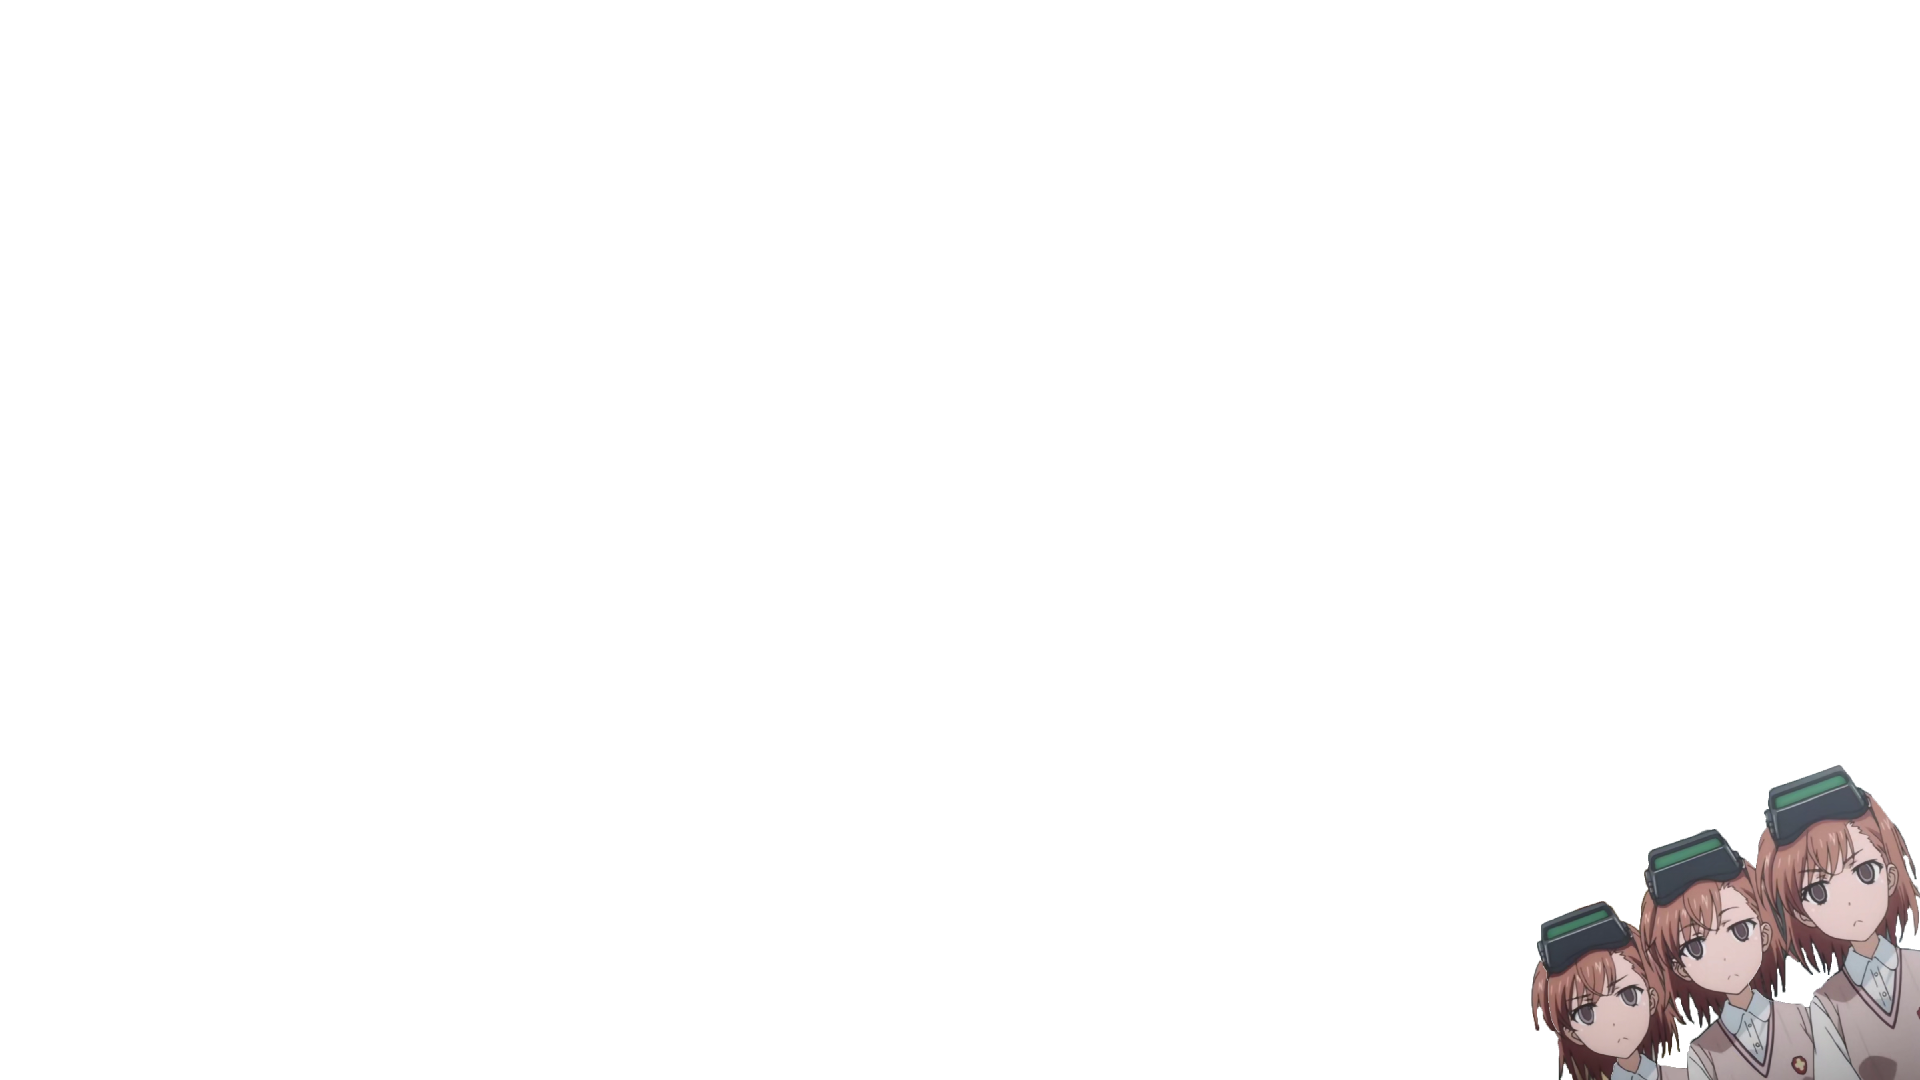
\includegraphics[height=\paperheight]{figures/sisters1080.png}}

\makeatletter 
\renewcommand{\@thesubfigure}{\hskip\subfiglabelskip}
\makeatother

\title{程序优化}
\author{施朱鸣}
\date{11月4日}

\begin{document}
    {
    % \setbeamertemplate{background}{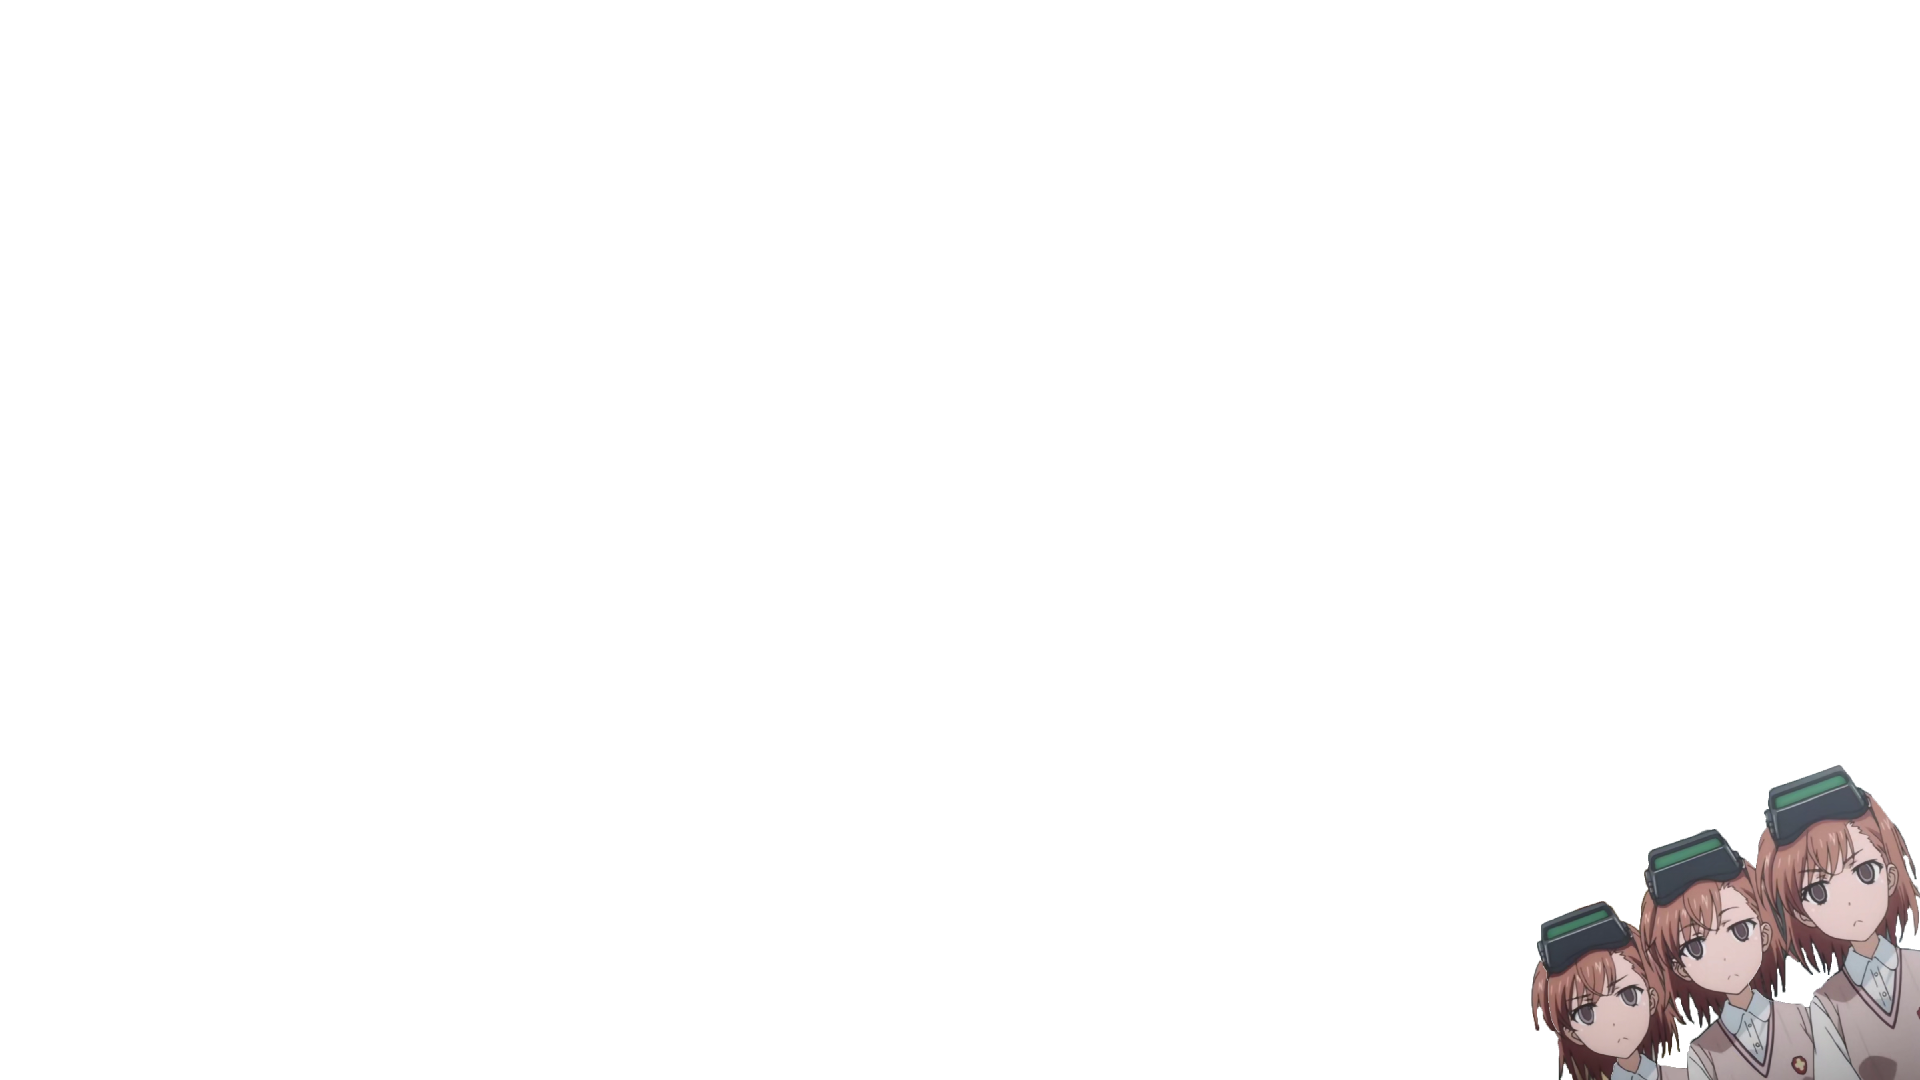
\includegraphics[height=\paperheight]{figures/sisters1080.png}}
    \setbeamertemplate{background}{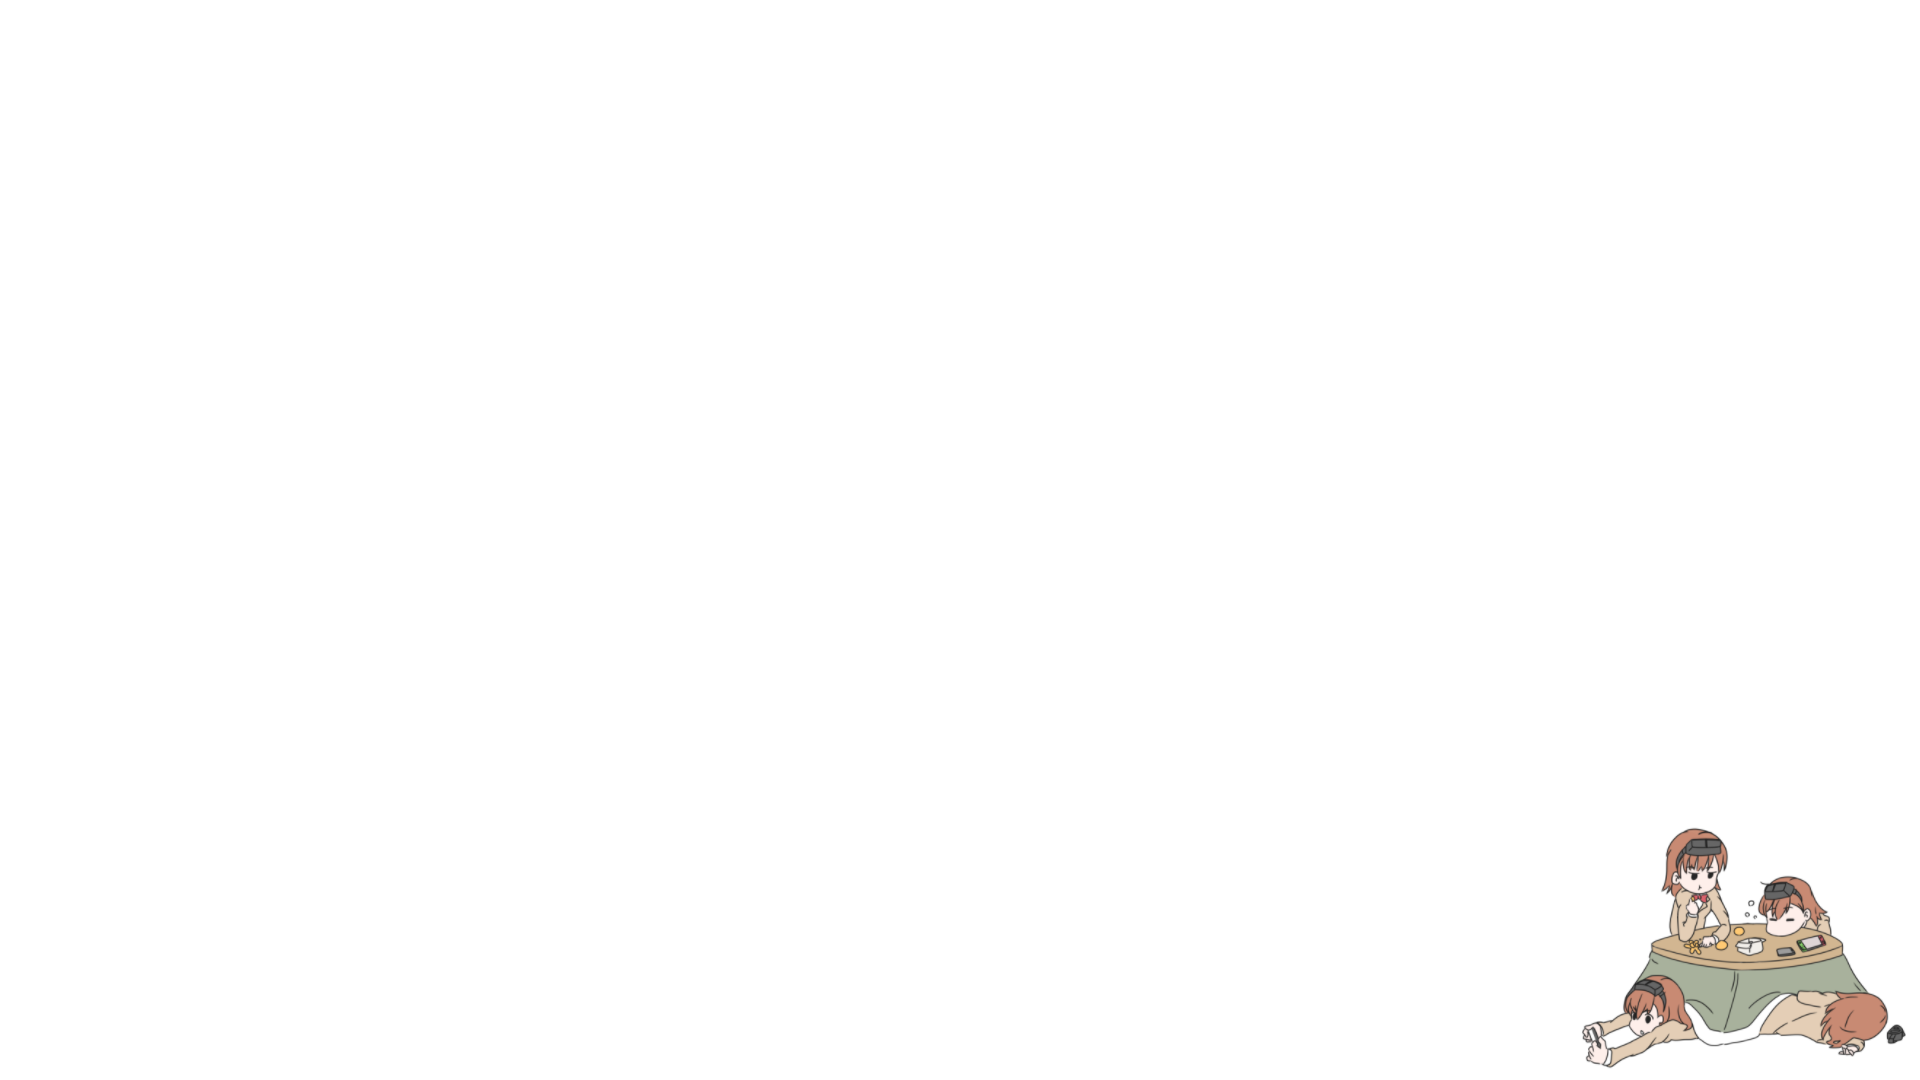
\includegraphics[height=\paperheight]{figures/misaka1080.jpg}}
    
    \begin{frame}
    \titlepage
    \end{frame}
    \frame{\frametitle{Outline}\tableofcontents[hideallsubsections]}

    \section{优化编译器}
    \begin{frame}
        \frametitle{减少重复计算同一个数}
    
        \begin{figure}
            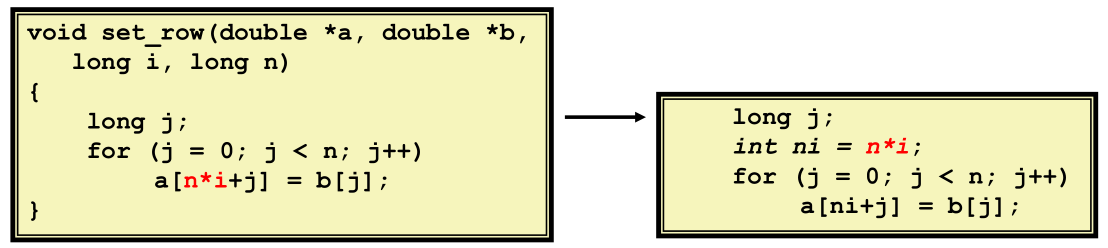
\includegraphics[width=\textwidth]{figures/1.png}
        \end{figure}
    
    \end{frame}

    \begin{frame}
        \frametitle{用简单的计算代替}
    
        乘除法开销大,视情况用累加或者位移运算实现
        \(16*x\rightarrow x<<4\)
        \begin{figure}
            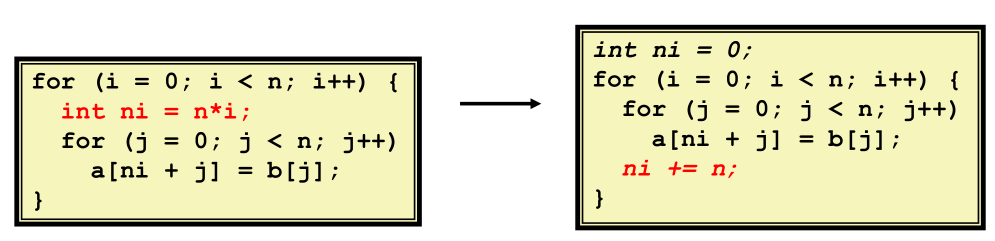
\includegraphics[width=\textwidth]{figures/2.png}
        \end{figure}
    
    \end{frame}

    \begin{frame}
        \frametitle{用简单的计算代替}
    
        分解复杂算式,把重复计算的数提出来
        \begin{figure}
            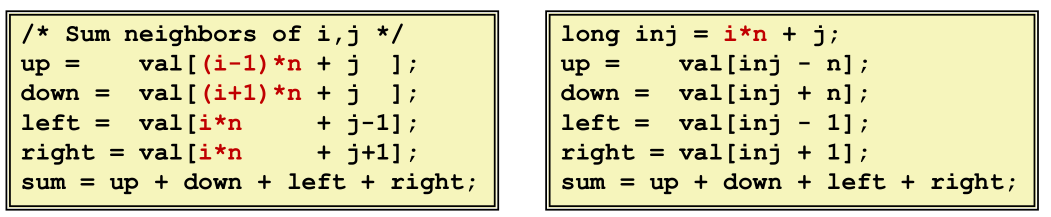
\includegraphics[width=\textwidth]{figures/3.png}
        \end{figure}
    
    \end{frame}

    \section{优化区块}

    \begin{frame}
        \frametitle{编译器优化的局限性}
    
        \begin{itemize}
            \item 为了不编译错,编译器只进行安全的优化
            \item 优化只在局部(procedures)进行
            \item 基于静态信息的优化
            \item 编译器不知道内存的实际情况
        \end{itemize}
    
    \end{frame}

    \begin{frame}
        \frametitle{消除低效率循环}
    
        编译器看不到跨越函数的情况,不敢优化

        “边带效应”:做了编译器没意识到的事情

        % 编译器:我不知strlen会造成什么影响,我很害怕

        \begin{figure}
            \subfigure[]{
                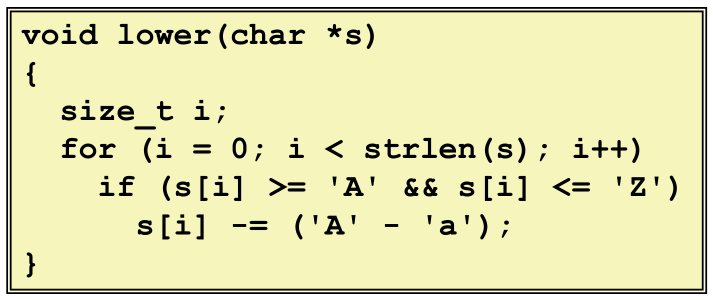
\includegraphics[width=.4\textwidth]{figures/4.png}
            }
            \subfigure[]{
                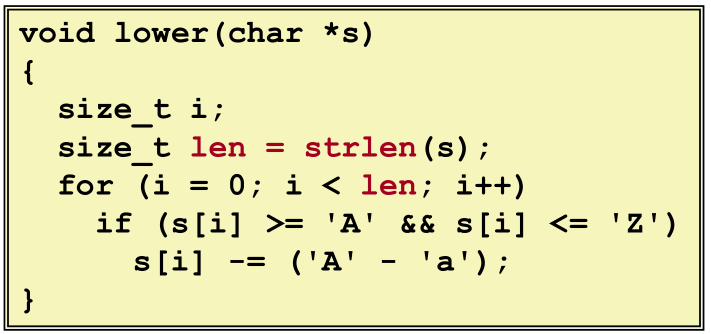
\includegraphics[width=.4\textwidth]{figures/5.png}
            }
        \end{figure}
    
    \end{frame}

    \begin{frame}
        \frametitle{消除不必要的访存}
    
        利用局部变量,但如果B和A相关可能会造成错误,编译器不敢优化

        \begin{figure}
            \subfigure[]{
                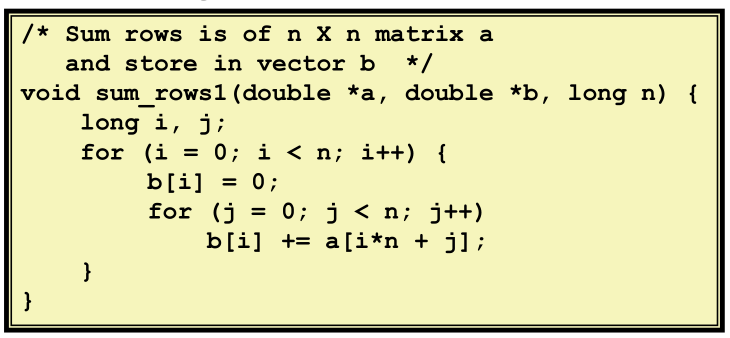
\includegraphics[width=.6\textwidth]{figures/6.png}
            }
            \subfigure[]{
                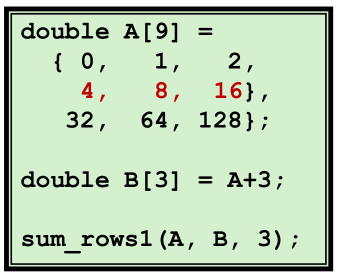
\includegraphics[width=.3\textwidth]{figures/7.png}
            }
        \end{figure}
    
    \end{frame}

    \begin{frame}
        \frametitle{减少不必要的访存}

        \begin{itemize}
            \item 一段内存有多个别名时,如果编译器进行优化可能发生错误,所以要人工进行优化。
            \item C中指针指来指去,编译器感到害怕
        \end{itemize}

    \end{frame}

    \section{处理器级优化}
    
    \section*{致谢}}

    \begin{frame}
        \setbeamertemplate{background}{}
        \frametitle{致谢}
        \begin{columns}
            \begin{column}{.5\linewidth}
                祝大家期中顺利,谢谢聆听!
            \end{column}
            \begin{column}{.5\linewidth}
                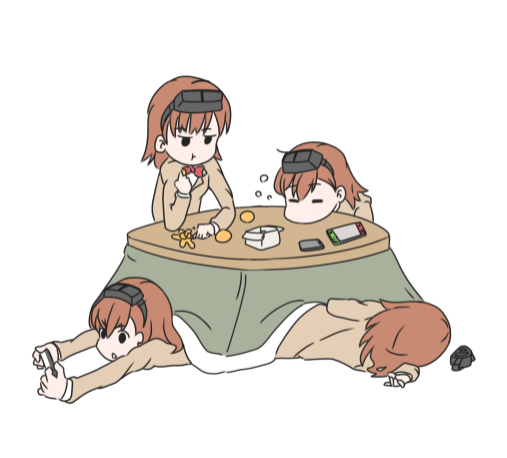
\includegraphics[width=.4\paperwidth]{figures/misaka558.png}
            \end{column}
        \end{columns}
    \end{frame}
    
\end{document}